\section{Performance of Annealing-based Quantum Computers}

\subsection{Hybrid DQM Solver}

For the optimization using the Quantum Annealing hardware, the formulated DQM is sent to a hybrid solver at D-Wave.
The hybrid solver does not put the DQM on quantum hardware directly.
It classically searches the solution space.
The hybrid solver speeds up this process by using quantum hardware to determine promising regions to explore next.
\cite{DQMHybrid2020}

The optimization of the DQM using the hybrid solver for small problems seems to have linear time complexity.
If the UCP grows by $10$ time instances, the optimization takes about $0.1$ seconds longer.
The results of the optimization and the time needed for the optimization are listed in table \ref{table:validation.annealing.performance}.
The optimization of these problems takes no longer than $5.6$ seconds each.

\begin{table}[ht]
  \centering
  \begin{tabular}{| r | r | r |}
  \hline 
  Number of Loads & Objective function & Time (in seconds) \\ 
  \hline \hline 
  10 & 487007.496 & 4.989 \\ \hline 
  20 & 817672.120 & 5.085 \\ \hline 
  25 & 681913.849 & 5.117 \\ \hline 
  30 & 1155685.053 & 5.215 \\ \hline 
  40 & 1554316.529 & 5.362 \\ \hline 
  50 & 1559508.051 & 5.510 \\ \hline 
\end{tabular}

  \caption{Results of Annealing Optimization with $4$ Power Plants}
  \label{table:validation.annealing.performance}
\end{table}

In figure \ref{figure:validation.annealing.performance} the time complexity is displayed clearer.
The time needed for optimizing problems with less than $15$ time instances also seems to be constant.
After that, the linear time complexity is clearly visible.

When the problem size increases, the time complexity seems to be worse than linear.
This becomes clear in figure \ref{figure:validation.annealing.performance.extended}.
The time taken by the hybrid solver to optimize the problem grows linearly but at a higher rate starting from $80$ time instances.
After this increase of slope, the slope stays the same until the problem size reaches $200$ time instances.
I did not test the optimization of problems with more than $200$ time instances on the D-Wave hardware.

\begin{figure}
  \begin{subfigure}[b]{0.5 \textwidth}
    \centering
    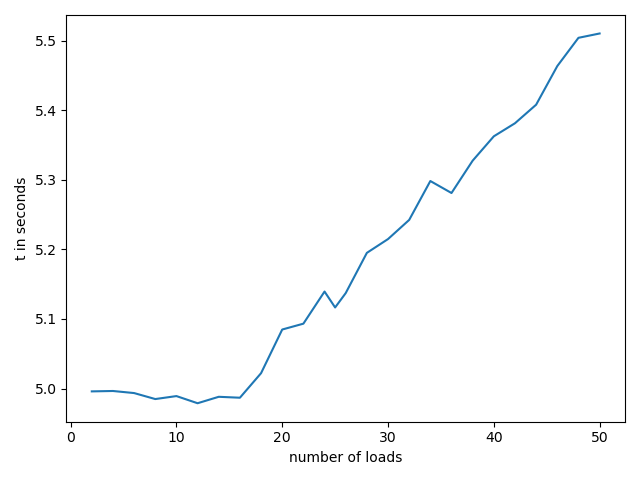
\includegraphics[width=\textwidth]{04_Validation/performance_annealing_p4.png}
    \caption{With up to $50$ Loads}
    \label{figure:validation.annealing.performance}
  \end{subfigure}
  \begin{subfigure}[b]{0.5 \textwidth}
    \centering
    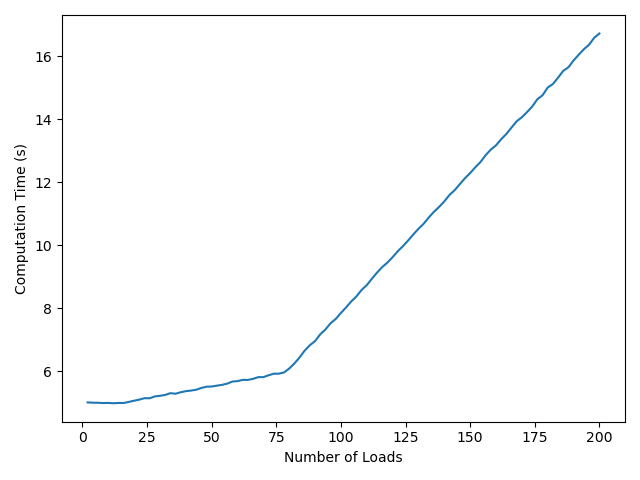
\includegraphics[width=\textwidth]{04_Validation/performance_annealing_p4_extended.png}
    \caption{With up to $200$ Loads}
    \label{figure:validation.annealing.performance.extended}
  \end{subfigure}
  \caption{Time Complexity of Annealing Optimization with $4$ Power Plants}
\end{figure}

After examining the computing time needed for the optimization of the DQMs by the hybrid solver, it gets clear that the hybrid solver uses the minimum time for each problem.
The hybrid DQM solver defines its minimum computing time with the pairs of density and time listed in table \ref{table:validation.dqm.hybrid.minimum.time}.
The solver chooses the minimum computing time for a given DQM by interpolating linearly between the nearest two points.
That gives a function that is shown in figure \ref{figure:validation.dqm.hybrid.minimum.time}.
Figure \ref{figure:validation.dqm.hybrid.minimum.time.200} shows the part of the function corresponding to the experimental data in figure \ref{figure:validation.annealing.performance.extended} with the same unit
--- number of time instances instead of density.
Notice how identical figure \ref{figure:validation.annealing.performance.extended} and figure \ref{figure:validation.dqm.hybrid.minimum.time.200} are.
\begin{table}[ht]
  \centering
  \begin{tabular}{| r | r |}
  \hline
  Density of DQM & Minimum Computing Time $t$ \\
  \hline \hline
  20000 & 5.0 \\
  \hline
  100000 & 6.0 \\
  \hline
  200000 & 13.0 \\
  \hline
  500000 & 34.0 \\
  \hline
  1000000 & 71.0 \\
  \hline
  2000000 & 152.0 \\
  \hline
  5000000 & 250.0 \\
  \hline
  20000000 & 400.0 \\
  \hline
  250000000 & 1200.0 \\
  \hline
\end{tabular}
  \caption{Interpolation Points for Minimum Computing Time of Hybrid DQM Solver}
  \label{table:validation.dqm.hybrid.minimum.time}
\end{table}
\begin{figure} [ht]
  \begin{subfigure}[b]{0.5 \textwidth}
    \centering
    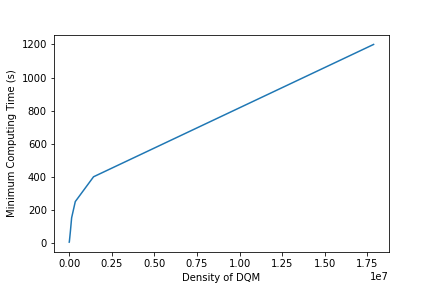
\includegraphics[width=\textwidth]{04_Validation/minimum_computing_time_dqm_hybrid.png}
    \caption{Full}
    \label{figure:validation.dqm.hybrid.minimum.time}
  \end{subfigure}
  \begin{subfigure}[b]{0.5 \textwidth}
    \centering
    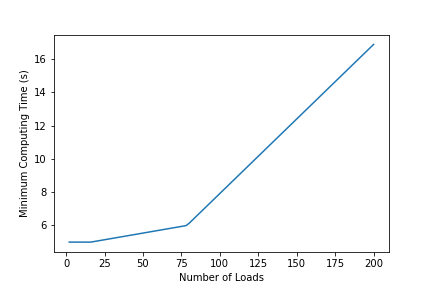
\includegraphics[width=\textwidth]{04_Validation/minimum_computing_time_dqm_hybrid_200.png}
    \caption{Corresponding to Extended Experiment Data}
    \label{figure:validation.dqm.hybrid.minimum.time.200}
  \end{subfigure}
  \caption{Minimum Computing Time of Hyvrid DQM Solver}
\end{figure}

This approach does not produce optimal solutions for the UCP.
The summed power output of the single power plants does not meet the power demand because the DQM underestimates the demand part of the UCP.
After retrieving the optimal DQM solution and translating it to a UCP solution, the program adjusts the power outputs of the power plants.
It does so as described in section \ref{approach:quantum.read.solution}.
That leads to a non-optimal solution of the UCP.

\subsubsection{Hybrid QUBO Solver}

This work implements the QUBOs for the UCP using the UQO-client.
The UQO-server, unfortunately, does not support the optimization of QUBOs using the hybrid solver.
For this reason, this work does not consider the performance of the hybrid solver for QUBOs.

\subsubsection{Direct QUBO Solver}

D-Wave's QPUs can embed many QUBOs on them.
But if a QUBO has too many variables or quadratic biases connecting the biases, D-Wave might not find an embedding.
That is the case for the problems this work considers.

The smallest problem formulated as a QUBO has $1, 024$ variables and $263, 680$ quadratic biases.
These values can be calculated using formulas (\ref{formula:qubo.num.variables}) and (\ref{formula:qubo.num.quadratic.biases}) respectively.
One variable can have more than $255$ quadratic biases, also called a clique.
The reason is that power plant $4$ has $2^8$ possible power levels after discretizing the power levels, and variables for the different power levels of one power plant at one time instances are connected with quadratic biases.

Since the ''Advantage'' QPU has a $15$-way qubit connectivity, it would need an enormous amount of physical qubits to represent one logical binary variable.
More as there are available on the ''Advantage'' QPU.
\cite{D-Wave2020, Zbinden2020}
Because of this, the minor miner can't find embeddings for the QUBOs this work considers.
An algorithm designed specifically for embedding large cliques by \citeauthor{Zbinden2020} can not embed cliques larger than $180$ for the ''Pegasus'' architecture.
\cite{Zbinden2020}
That implies that it is generally very hard or even impossible to find embeddings for QUBOs with cliques larger than $255$.
